\subsection{Level3.1: パラメータのチューニング}
\subsubsection{最適なパラメータを探すためのアプローチ}
最適なパラメータを探すために,3つのパラメータをそれぞれを探索するスクリプトを作成した.
\begin{itemize}
	\item HIDDEN.sh :HIDDENの値を1ずつ書き換えながら平均値を出力
	\item ALPHA.sh  :引数に「ALPHAの初期値」「ALPHAの刻み値」「ALPHAの最大値」を取り,連続的に実行する.
	\item ETA.sh    :ALPHA.shと同様にETAを小刻みに変更しながら実行を行う.
\end{itemize}

\subsubsection{実行結果}
\begin{itemize}
	\item HIDDEN
	\item ETA:
	\item ALPHA:
\end{itemize}<++>

\begin{table}[htb]
 \begin{center}
  \caption{階層型NNによる文字認識問題の学習に要した回数}
  \label{table:level3}
  \begin{tabular}[htb]{r|l} \hline
   シード値 & 収束した回数 \\ \hline \hline
   100 & hoge \\ \hline
   200 & hoge \\ \hline
   300 & hoge \\ \hline
   400 & hoge \\ \hline
   500 & hoge \\ \hline
   600 & hoge \\ \hline
   700 & hoge \\ \hline
   800 & hoge \\ \hline
   900 & hoge \\ \hline
   1000 & hoge \\ \hline \hline
   10試行の平均値 & hoge \\ \hline
  \end{tabular}
 \end{center}
\end{table}

\begin{figure}[h]
 \begin{center}
  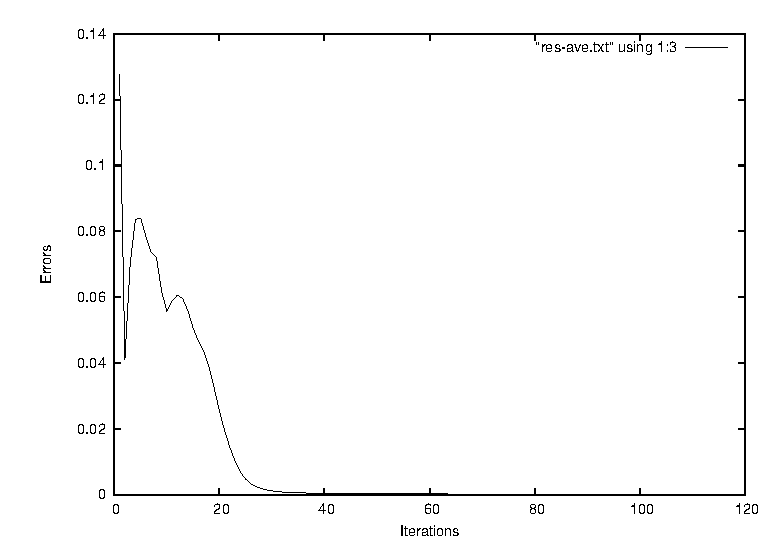
\includegraphics[width=10.0cm]{figs/sample2.eps}
  \caption{重みを更新する様子(平均値)}
  \label{fig:level2}
 \end{center}
\end{figure}


\subsubsection{考察}


